\chapter{Teorie del legame chimico}

\begin{quote}
    ``It is structure that we look for when we try to understand everything''.
    \begin{flushright}
    \textit{- L. Pauling}
    \end{flushright}
\end{quote}
In generale, il legame dei solidi può essere classificato in quattro grandi categorie:
\begin{enumerate}
    \item Van der Waals, tipico dei
    gas nobili e dei sistemi caratterizzati da gusci di valenza chiusi;
    \item ionico, osservato tra elementi diversi caratterizzati da valori di elettronegatività molto diversi fra loro;
    \item covalente, caratteristico di elementi con valori di elettronegatività relativamente grandi;
    \item metallico.
\end{enumerate}
\section{Legame ionico}
Si considerino gli elementi del VII gruppo. Questi elementi si trovano agli estremi della tavola periodica e sono caratterizzati da valori molto diversi di elettronegatività, energia di ionizzazione e affinità elettronica. Consideriamo ad esempio un atomo di litio e uno di fosforo. Il primo ha una bassa energia di ionizzazione e bassa elettronegatività, mentre il secondo ha un'elevata affinità elettronica e alta elettronegatività. Sulla base di queste osservazioni è naturale pensare che l'interazione tra atomi di litio e fluoro porti alla ionizzazione del primo, con formazione di un catione carico positivamente $\text{Li}^+$ con configurazione elettronica corrispondente a quella dell' elio, e alla formazione di ioni $\text{F}^-$ con configurazione elettronica corrispondente a quella del Ne, secondo la reazione $\ce{Li}+\ce{F}\to\ce{Li+} + \ce{F-}$. Questo stato di cose rappresenta un caso limite e il legame che ne deriva è indicato come legame ionico.
\begin{defn}[legame ionico]
     Legame chimico di natura elettrostatica che si forma quando gli atomi possiedono un'elevata differenza di elettronegatività, ovvero una bassa energia di ionizzazione e un'alta affinità elettronica.
\end{defn}
La formazione del legame corrisponde a un trasferimento pressoché completo dell'elettrone di valenza del litio all'atomo di fluoro, risultante in una coppia $\text{Li}^+\text{F}^-$. I due ioni sono stabili e possono essere trattati come due cariche nette di segno opposto che si attraggono secondo la legge di Coulomb. Naturalmente gli ioni litio e fluoruro non sono semplicemente due cariche di segno opposto in quanto sono presenti in entrambi i casi elettroni dei gusci interni. La formazione del legame chimico che in questo caso viene indicato come legame ionico, comporta la minimizzazione dell'energia complessiva del sistema raggiungendo una situazione di stabilità in cui forze di
attrazione e forze di repulsione si bilanciano.
\begin{figure}[ht]
    \centering
    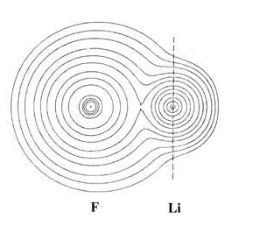
\includegraphics[width=0.4\linewidth]{Immagini/LiF.png}
    \caption{Coppia ionica LiF.}
    \label{fig:LiF}
\end{figure}

Si consideri un catione e valutiamo l'andamento dell'energia in funzione della distanza $r$. L'energia di interazione sarà data dalla somma dei termini attrattivi $V_{att}$ e repulsivi $V_{rep}$.
Il potenziale complessivo $V_{TOT}$ sarà dato dalla somma dei due contributi
\begin{equation}
    V_{TOT}=\frac{-e^2}{4\pi\varepsilon_0r}+\frac{b}{r^n}.
\end{equation}
Ad un certo valore critico di $r$, $r_0$, le forze attrattive e repulsive si bilanciano e il sistema è in equilibrio, ovvero la forza netta è zero. A questa distanza critica corrisponde un minimo energetico. Questo minimo di energia rappresenta l'energia di legame $E_l$ e la distanza $r_0$ è la distanza di legame. Considerando che $E_l$ corrisponde
ad un minimo di $V_{TOT}$
\begin{equation}
    \frac{\partial V_{TOT}}{\partial r}\bigg|_{r=r_0}=\frac{e^2}{4\pi\varepsilon_0 r_0^2}-\frac{nb}{r^{n+1}}=0.
\end{equation}
Moltiplicando ambo i membri per $r_0^2$ si ottiene
\begin{equation}
    \frac{e^2}{4\pi\varepsilon_0}-\frac{nb}{r^{n-1}}=0,
\end{equation}
da cui
\begin{equation}
\label{eq: raggio legame ionico}
    r_0=\left(\frac{4\pi\varepsilon_0nb}{e^2}\right)^{\frac{1}{n-1}}=r_{cat} + r_{an}.
\end{equation}
L'equazione \eqref{eq: raggio legame ionico} fornisce la distanza di legame della coppia ionica, ovvero la distanza alla quale le forze di attrazione sono bilanciate da quelle di repulsione e non vi è forza netta sui nuclei. Invece, per valutare l'energia di legame $E_l$ si calcola
\begin{equation}
    \frac{1}{n}=\left(\frac{4\pi\varepsilon_0b}{e^2 r^{n-1}}\right).
\end{equation}
Ora
\begin{equation}
    E_L=V_{TOT}^{r_0}=\frac{-e^2}{4\pi\varepsilon_0r_0}-\frac{b}{r_0^n}\Rightarrow E_L=\frac{-e^2}{4\pi\varepsilon_0r_0} \left(1-\frac{4\pi\varepsilon_0r_0b}{e^2 r_0^n}\right).
\end{equation}
Sostituendo il risultato trovato per $1/n$ si trova 
\begin{equation}
    E_L=\frac{-e^2}{4\pi\varepsilon_0r_0}\left(1-\frac{1}{n}\right).
\end{equation}
Nel
caso più generale in cui la carica degli ioni sia maggiore di 1 l'energia di legame diventa
\begin{equation}
    E_L=-\frac{Z^+Z^-e^2}{4\pi\varepsilon_0r_0}\underbrace{\left(1-\frac{1}{n}\right)}_{\substack{potenziale\\repulsivo\\di\,Born}},
    \label{eq:en.reticolare}
\end{equation}
dove $Z^+$ e $Z^-$ sono le cariche dell'anione e del catione rispettivamente.
\begin{figure}[h]
    \centering
    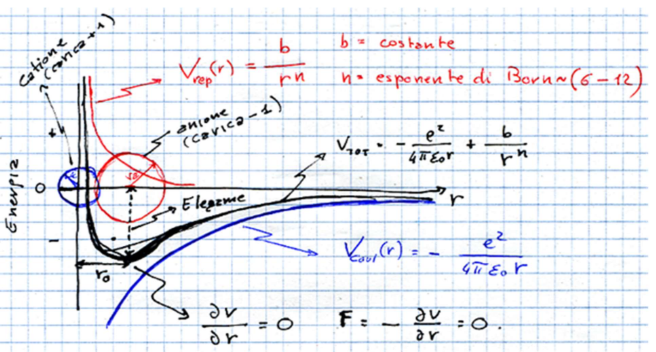
\includegraphics[width=0.5\linewidth]{Immagini/Grafico energia potenziale in funzione della distanza per due ioni di carica unitaria opposta.png}
    \caption{Energia potenziale in funzione di $r$.}
    \label{fig:en.pot.}
\end{figure}

\subsubsection{Energia reticolare}
Le sostanze ioniche non si trovano in forma di molecole ma in forma di aggregati cristallini in cui cationi e anioni sono organizzati in reticoli tridimensionali. Si dimostra ora che l'energia di un numero di Avogadro $N_A$ di coppie ioniche isolate è maggiore di quella di un $N_A$ di ioni disposti in un filare monodimensionale. L'energia di un $N_A$ di coppie ioniche non interagenti è data dall'equazione \eqref{eq:en.reticolare} moltiplicata per $N_A$
\begin{equation}
    E_L=-\frac{N_AZ^+Z^-e^2}{4\pi\varepsilon_0r_0}\left(1-\frac{1}{n}\right).
\end{equation}
Si confronta ora questa energia con quella del filare di $N_A$ ioni positivi e negativi data dal termine coulumbiano
\begin{align}
\label{eq: energia formazione reticolo}
        \begin{split}
        E_C&=\frac{N_AZ^+Z^-e^2}{4\pi\varepsilon_0}\left(-\frac{2}{r_0}+\frac{2}{2r_0}-\frac{2}{3r_0}+\frac{2}{4r_0}+\cdots\right) \\ 
        &=\frac{N_AZ^+Z^-e^2}{4\pi\varepsilon_0}\frac{2}{r_0}\left(-1+\frac{1}{2}-\frac{1}{3}+\frac{1}{4}+\cdots\right) \\
        &=\frac{N_AZ^+Z^-e^2}{4\pi\varepsilon_0}\frac{2}{r_0}\underbrace{\sum_{n=1}^{\infty}\frac{\left(-1\right)^{n}}{n}}_{=-0.693}. 
   \end{split}
\end{align}
Quindi,l'equazione \eqref{eq: energia formazione reticolo} dimostra che  la formazione di un reticolo monodimensionale diminuisce l'energia del sistema di un fattore $-1.386$.  Considerando un reticolo tridimensionale si ottiene un valore ancora inferiore che nel caso di un sistema cubico a facce centrate come $\text{NaCl}$ è pari a $-1.748$. Questo termine è una costante che dipende esclusivamente da come sono disposti gli ioni nel reticolo e prende il nome di costante di Madelung. L'energia reticolare complessiva di un cristallo ionico, considerando anche il potenziale di Born, è data dall'equazione di Born-Landé
\begin{equation}
    E_R=-\frac{MN_AZ^+Z^-e^2}{4\pi\varepsilon_0r_0}\left(1-\frac{1}{n}\right).
\end{equation}

\subsubsection{Ciclo di Born-Haber}
L'energia reticolare può essere misurata sperimentalmente attraverso un ciclo termodinamico ricordandoche la variazione di entalpia $\Delta H$ in una reazione chimica è indipendente dal percorso o numero di stadi in cui avviene il processo (Legge di Hess). 

Si consideri la formazione di \text{NaCl}. L'energia reticolare corrisponde al calore di formazione di una mole di \text{NaCl} a partire dai suoi costituenti in fase gas
\begin{equation}
    \textnormal{Na}_{\left(g\right.)}^++\frac{1}{2}\textnormal{Cl}_{2\left(g)\right.}^-\to \textnormal{NaCl}_{\left(s\right.)}.
\end{equation}
Questa energia non può essere misurata sperimentalmente, tuttavia il calore di formazione di un cristallo può essere misurato relativamente ai reagenti nei loro stati standard 
\begin{equation}
    \textnormal{Na}_{\left(s\right.)}+\frac{1}{2}\textnormal{Cl}_{2\left(g)\right.}\to \textnormal{NaCl}_{\left(s\right.)},\qquad\Delta H=\Delta H_f.
\end{equation}
La quantità $\Delta H_f$ può essere messa in relazione all'energia reticolare $E_R$ costruendo un ciclo termodinamico di Born-Haber in cui $\Delta H_f$ è dato dalla somma dei termini energetici di diversi stadi ipotetici. In particolare, per \text{NaCl} gli stadi sono: la sublimazione di \text{Na} metallico; la ionizzazione di \text{Na} gas; la dissociazione della molecola $\text{Cl}_2$; la formazione dello ione cloruro $\text{Cl}^-$; l'energia di formazione del reticolo $E_R$. I quali sommati restituiscono $\Delta H_f$. 

\section{Legame covalente}
L'opposto del legame ionico è quello relativo al legame tra due atomi dello stesso tipo come ad esempio nel caso della molecola di idrogeno. Anche in questo caso la forza che tiene legati i nuclei sarà di natura elettrostatica. Rispetto al caso precedente però la distribuzione di densità elettronica sarà omogenea sui due atomi costituenti la molecola. In generale la densità elettronica può essere pensata come una nuvola o un gas di carica negativa che varia la propria densità nella molecola. Il caso è più complesso di quello precedentemente descritto e può essere trattato solo attraverso l'approccio quanto meccanico. L'energia degli elettroni in una molecola è quantizzata così come lo è negli atomi . Anche nel caso delle molecole i nuclei possono essere considerati stazionari rispetto al moto degli elettroni. Per una certa distanza internucleare $R$, ci sono una serie di livelli energetici permessi. La distribuzione della densità elettronica per la molecola di idrogeno può essere illustrata attraverso una mappa di isodensità elettronica. Si immagini una molecola di idrogeno tagliata a metà lungo un piano che contiene i nuclei. La quantità di carica elettronica in ciascun punto nello spazio è determinata e tutti i punti con lo stesso valore di densità elettronica nel piano sono uniti
da una linea continua.
\begin{figure}[h]
    \centering
    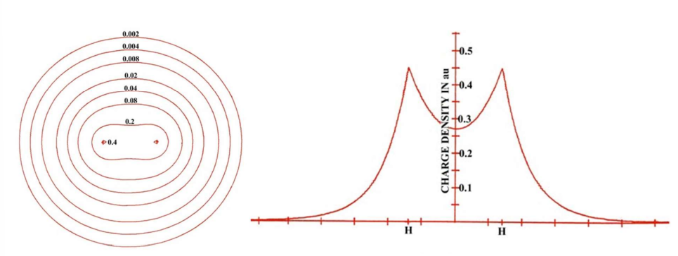
\includegraphics[width=0.7\linewidth]{Immagini/mappa densità elettronica H2.png}
    \caption{mappa densità elettronica \textnormal{H}$_2$.}
    \label{fig:Mappa densità elettronica $H_2$}
\end{figure}
La figura ci mostra come ci sia nella molecola un accumulo di densità di carica nella regione internucleare e come in generale la distribuzione di densità elettronica sia modificata rispetto a quella dell'atomo libero, che si concentra nella regione di legame.

La semplice sovrapposizione della densità elettronica delle specie atomiche non giustifica la formazione del legame e come sia necessario un incremento di densità elettronica tra i nuclei per bilanciare le forze di repulsione internucleare. Le regioni in cui la densità di carica elettronica aumenta nella mappa di differenza di densità di carica, sono quindi le regioni in cui la carica elettronica è trasferita rispetto agli atomi separati in modo da ottenere uno stato di equilibrio elettrostatico e quindi un legame chimico. A separazioni grandi, la distribuzione di densità elettronica in ciascun atomo è polarizzata nella direzione dell'altro atomo e una piccola quantità di densità di carica è trasferita dalla regione al di fuori dei nuclei a quella interna. Questa regione è indicata di legame, mentre la regione di spazio in cui c'è un depauperamento della densità elettronica è indicata come regione di antilegame. Questo indica che anche a distanza molto grandi le distribuzioni atomiche non sono più sferiche. 
\begin{figure}[ht]
    \centering
    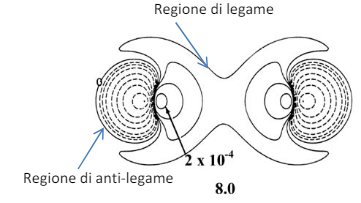
\includegraphics[width=0.6\linewidth]{Immagini/Distribuzione densità elettronica H2.png}
    \caption{Distribuzione densità elettronica \textnormal{H}$_2$ a 8 au.}
    \label{fig:distribuzione densità elettronica $H_2$}
\end{figure}

Questa distorsione nella
distribuzione di densità elettronica (polarizzazione) comporta un incremento (anche se piccolo) della forza
attrattiva. Queste forze attrattive che agiscono a distanza sono note come forze di dispersione o di van der Waals.

Il principio di esclusione di Pauli gioca un ruolo importante nel determinare la struttura molecolare. Nel caso di un atomo il principio di Pauli richiede che elettroni confinati nella stessa regione di spazio (ovvero nello stesso orbitale) devono avere I loro spin appaiati. Questo è vero anche nel caso della formazione del legame tra due atomi in una molecola. Si considerino due atomi di idrogeno che si avvicinano uno all'altro. Quando sono relativamente vicini tra di loro gli elettroni diventano indistinguibili e non è più possibile dire quale di essi è associato a quale atomo, poiché entrambi si muovono nei pressi dei due nuclei. Come già visto, questa è la condizione perché si formi il legame. Tuttavia, perché i due elettroni possano essere confinati in questa regione limitata di spazio i loro spin devono necessariamente essere appaiati. Nella regione di legame un elettrone tenderà ad escludere la presenza dell'altro se i loro spin sono paralleli e all'avvicinarsi dei due nuclei la densità di carica sarà rimossa dalla regione di legame e allocata nella regione di antilegame (dietro I nuclei) dando origine ad
un'interazione repulsiva.
\begin{obs}[linee guida generali per la formazione del legame chimico]
    Densità elettronica dev'essere accumulata nella regione internucleare in misura maggiore a quanto si può
    ottenere per la semplice sovrapposizione delle densità elettroniche atomiche. In generale l'incremento di
    densità di carica elettronica necessario a bilanciare la repulsione internucleare richiede due elettroni.
\end{obs}
\subsection{Strutture di Lewis}
A differenza dell'idrogeno, gli atomi di elio nel loro stato fondamentale non possono legarsi a nessun atomo neutro per formare una molecola.  Quando due atomi di elio si avvicinano ciascun elettrone del primo atomo ne incontra un altro, associato al secondo, che ha lo stesso spin. Per il principio di Pauli, nessuno degli elettroni può concentrare la sua densità nella regione internucleare. Questa densità verrà pertanto distribuito nella regione di antilegame. Il fatto che sia il principio di Pauli a prevenire la formazione del legame nella molecola di $\text{He}_2$ è evidente dal fatto che $\text{He}_2^+$, che possiede un elettrone in meno è stabile. Tutti i gas nobili possiedono una struttura a guscio chiuso e questo spiega la loro inerzia chimica. Non esistono molecole biatomiche omonucleari, tutti sono presenti in natura come gas monoatomici. Solo un elemento con un'elevata affinità elettronica può formare un legame con un gas nobile. L'unica specie con un'affinità elettronica sufficiente a legare un atomo di \text{He} è lo ione $\text{He}^+$. Se l'atomo di \text{He} ha la più alta energia di ionizzazione, lo ione $\text{He}^+$ dovrà possedere la maggior affinità elettronica. 
\begin{obs}[ibridazione del carbonio]
    La configurazione elettronica del carbonio è $1s^22s^22p^2(\uparrow\uparrow)$. Ci si aspetta quindi la formazione di due legami. Eppure, questo va contro l'evidenza sperimentale della stabilità della molecola di metano $\text{CH}_4$, dove si formano quattro legami covalenti identici con quattro atomi di idrogeno. Questo fatto può essere spiegato considerando che la differenza in energia tra gli orbitali 2s e 2p non è molto elevata. La distribuzione elettronica di \text{C} quindi si riorganizza dando luogo ad una nuova in cui si formano quattro livelli energetici ognuno con la stessa energia e contenente un elettrone (ibridazione). L'energia richiesta per passare dalla configurazione atomica più stabile a questa è più che compensata dal guadagno energetico ottenuto formando altri due legami \text{C-H}. Tale riorganizzazione, delle funzioni d'onda dell'orbitale, è matematica, e non corrisponde ad un reale fenomeno fisico.
\end{obs}
Un ottimo modo per rappresentare atomi, i legami tra essi, molecole e ioni, sono le strutture di Lewis.
\begin{axiom}[strutture di Lewis]
    Una generica struttura di Lewis si costruisce seguendo lo schema:
    \begin{enumerate}
        \item si contano il numero di elettroni di valenza totali a partire dalla formula molecolare;
        \item si pone l'elemento più elettronegativo al centro della struttura e all'esterno quelli con elettronegatività minore, con particolare agli idrogeni che devono sempre essere in posizione più esterna;
        \item si completano gli ottetti degli atomi più esterni, per poi completare quello dell'atomo centrale con gli elettroni rimanenti;
        \item se l'atomo centrale non possiede l'ottetto completo e non sono più disponibili elettroni, è possibile che siano presenti legami doppi o tripli;
        \item si verifica che il numero ed il modulo delle cariche formali sia il minore possibile ed inoltre che cariche formali positive non si trovino su elementi elettronegativi.
    \end{enumerate}
\end{axiom}
\begin{defn}[legame $\sigma$]
    Un legame di tipo $\sigma$ avviene tra due atomi che mettono in comune un elettrone ciascuno e si forma con la sovrapposizione dei due orbitali frontalmente.
\end{defn}
\begin{defn}[legame $\pi$]
    Un legame di tipo $\pi$ si forma con la sovrapposizione laterale di due orbitali di opportuna simmetria.
\end{defn}
Ciascuna riga corrisponde a due elettroni localizzati nella regione di spazio tra I due atomi. Moltiplicando per
due il numero di righe e aggiungendo I rimanenti elettroni di valenza indicati ciascuno da un puntino si ottiene
il valore di 8 nella grande maggioranza dei casi (esistono alcune eccezioni) e in particolare per gli elementi
del secondo periodo. Questo numero corrisponde al numero massimo di elettroni che possono essere allocati
nel guscio di valenza.
\begin{obs}[regola dell'ottetto]
    Il raggiungimento di questa configurazione non
è la forza che guida il processo, ma semplicemente il risultato della configurazione elettronica degli
elementi.
\end{obs}

\paragraph{Gusci espansi.} Quando è impossibile disegnare una struttura di Lewis coerente con la regola dell'ottetto, è necessario aumentare il numero di elettroni attorno all'atomo centrale. Un'opzione limitata ad elementi del terzo periodo è quella di usare orbitali d per giustificare questa espansione.
\begin{ex}($\text{ClF}_3$ e $\text{SF}_6$)
    Le molecole di $\text{ClF}_3$ e $\text{SF}_6$ hanno strutture di Lewis con guscio espanso. L'aumentato numero di elettroni viene descritto attraverso l'immagine di un guscio espanso. Questa espansione corrisponde ad utilizzare gli stati $3d$ vuoti che nel terzo gruppo hanno energie non troppo distanti da quelli degli orbitali $3p$.
\end{ex}

\subsection{Legame covalente polare}
La densità elettronica può essere convenientemente immaginata come una nuvola o un gas carico negativamente che varia la sua densità attraverso la molecola. Se i due atomi che costituiscono una semplice molecola biatomica non sono però identici la densità elettronica non sarà distribuita in maniera omogenea sui due atomi ma tenderà ad accumularsi nei pressi dell'elemento più elettronegativo. Il legame ionico e covalente rappresentano i due possibili estremi per raggiungere uno stato di equilibrio elettrostatico e c'è un intero spettro di distribuzioni di densità all'interno di questi due estremi associata alle diverse elettronegatività degli atomi costituenti. Le conseguenze di una distribuzione non omogenea di densità elettronica comportano una serie di conseguenze importanti: la presenza di un momento di dipolo netto e l'incremento dell'energia di legame. 

Si consideri il caso della molecola HF. La differenza di elettronegatività tra H e F è di 1.39, elevato ma minore di quella tra Li e F di 3.28. Pertanto, HF è una molecola neutra in cui la distribuzione di carica è asimmetrica, polarizzata verso F. Una tale distribuzione comporta l'insorgenza di un momento di dipolo elettrico permanente $\bm{P}$, diretto verso dalla carica negativa a quella positiva. visti questi piccoli valori per sistemi molecolari si usa come unità il Debye ($1\text{D}=3.336\times10^{-30}\,\text{C}\cdot \text{m}$). Per HF è di 1.9 D, per LiF è di 6.0 D. Questa grande differenza indica chiaramente che la separazione di carica all'interno della molecola di HF è nettamente minore di quella presente nella molecola di LiF che è pressoché totale.
\begin{figure}[h]
    \centering
    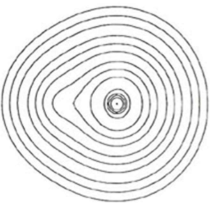
\includegraphics[width=0.3\linewidth]{Immagini/HF.png}
    \caption{mappa di densità elettronica \textnormal{HF}.}
    \label{fig:HF}
\end{figure}
\begin{obs}[calcolo momento di dipolo]
    Numericamente si calcola che il momento di dipolo di LiF è di 7.34 D. Questa differenza dal valore sperimentale (6.0 D) sta nell'approssimazione che le cariche siano sfere rigide.
\end{obs}
La differenza di elettronegatività fornisce una guida importante per valutare non solo il fatto che una
molecola sia polare ma anche per stimare la carica parziale presente su due atomi all'interno di una molecola
polare.
\begin{defn}[carica parziale]
    Una carica parziale su un atomo è una carica che ha un valore inferiore a 1. Indica quindi che gli elettroni condivisi di un legame covalente sono distribuiti in modo non omogeneo.
\end{defn}
E' possibile
stimare la carica parziale usando un'equazione proposta da Allen.
\begin{axiom}[carica parziale di Allen]
    Data una molecola biatomica AB, i cui atomi costituenti hanno elettronegatività $\chi_A\neq\chi_B$, la carica parziale $\delta_A$ sull'atomo A è data da
    \begin{equation}
        \delta_A=G_A - L_A -B\left(\frac{\chi_A}{\chi_A + \chi_B}\right),
        \label{eq:carica formale}
    \end{equation}
    dove $G_A$ è il numero di elettroni di valenza di A, $L_A$ è il numero di
elettroni di valenza non impegnati nel legame su A e $B$ è il numero di elettroni di
legame. 
\end{axiom}
\begin{ex}
    Nel caso si \textnormal{HF} si ha
    \begin{equation}
        \begin{cases}
            \delta_F=7-6-2\left(\dfrac{4.19}{4.19+2.3}\right)=-0.29 \\[2ex]
            \delta_H=1-0-2\left(\dfrac{2.3}{4.19+2.3}\right)=+0.29,
        \end{cases}
    \end{equation}
    da cui si trova per \textnormal{HF} un momento di dipolo $\bm{P}=1.3\,D$, in ragionevole accordo con il valore sperimentale $\bm{P}=1.94\,D$.
\end{ex}
In questi casi il legame è indicato come covalente-polare e la polarità del legame aumenta all'aumentare della differenza di elettronegatività. Valori estremi di $\Delta\chi$ coincidono con una separazione netta di carica e formazione del legame ionico. 

\subsection{Teoria VSEPR}
Determinare la geometria molecolare è estremamente importante dal momento che questa determina molte delle proprietà fisiche e chimiche. La geometria molecolare può essere prevista in maniera semplice considerando la repulsione tra coppie elettroniche dovuta al principio di Pauli. Questa teoria sviluppata da R. J. Gillespie è nota come VSEPR (Valence Shell Electron Pair Repulsion) ed è basata sulla seguente assunzione.
\begin{axiom}[principio della teoria VSEPR]
    La distribuzione di densità elettronica nei gusci di valenza di atomi in molecole è determinata principalmente dalle repulsioni tra coppie di elettroni generate dal principio di Pauli.
\end{axiom}
Pertanto, segue che la posizione degli elettroni può essere dedotta basandosi sugli spin degli stessi.
\begin{axiom}[posizione degli elettroni nella teoria VSEPR]
    Due elettroni con spin parallelo avranno la massima probabilità di trovarsi ai lati opposti del nucleo, tre elettroni ai vertici di un triangolo equilatero, quattro elettroni in corrispondenza dei vertici di un tetraedro e così via.
\end{axiom}
\begin{figure}[h]
    \centering
    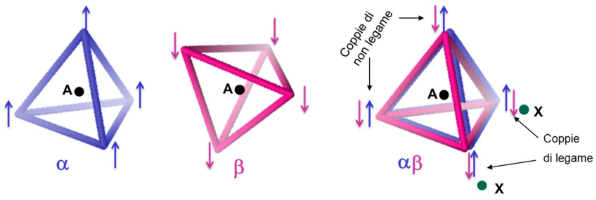
\includegraphics[width=0.8\linewidth]{Immagini/Distribuzione elettroni VSEPR.png}
    \caption{distribuzione degli elettroni per la teoria VSEPR.}
    \label{fig:VSEPR}
\end{figure}

Ciascuno degli arrangiamenti di un dato numero di coppie elettroniche può dare origine a diverse geometrie molecolari a seconda del numero di coppie di legame e coppie di non legame. La seguente terminologia è utile.
\begin{notz}
    Nella teoria VSEPR si indica con:
    \begin{enumerate}
        \item A l'atomo centrale.
        \item X un atomo legato ad A.
        \item E una coppia di non legame.
    \end{enumerate}
    In una generica molecola $\text{AX}_m\text{E}_n$ ci sono $(m+n)$ coppie di elettroni nel guscio di valenza, di cui $m$ sono coppie di legame e $n$ sono coppie di non legame. La forma della molecola è determinata dell'organizzazione delle $(m+n)$ coppie elettroniche.
\end{notz}
Molti dettagli fini della struttura molecolare possono essere capiti sulla base delle seguenti considerazioni. 
\begin{corl}
Dal fatto che coppie elettroniche tendono a respingersi e ad occupare regioni di spazio le più distanti possibili si deduce che:
    \begin{enumerate}
        \item Coppie di elettroni di non-legame respingono coppie elettroniche adiacenti in maniera maggiore delle
        coppie di legame. 
        \item Le repulsioni esercitate da una coppia di legame diminuiscono con l'aumentare dell'elettronegatività
        dell'atomo esterno. 
        \item Legami multipli esercitano repulsioni maggiori rispetto a legami singoli. 
        \item Le repulsioni tra coppie elettroniche in gusci chiusi sono maggiori di quelle tra coppie di elettroni in
        gusci incompleti.
    \end{enumerate}
\end{corl}

\subsection{Composti che non esistono}
Sulla base delle considerazioni fatte fino ad ora è interessante cercare di razionalizzare il fatto che ci sia una varietà di composti le cui strutture pur non offendendo le semplici regole della valenza, sono caratterizzati da una forte instabilità.

Alcuni composti sono instabili a causa delle restrizioni imposte dalla configurazione eletronica di valenza. Il guscio di valenza degli elementi del secondo periodo può accomodare al massimo otto elettroni negli orbitali $2s$ e $2p$. La formazione di più di 4 legami da parte di questi elementi richiederebbe l'uso di orbitali 3d che sono però ad energie troppo elevate rispetto a quelli del livello quantico caratterizzato da $n=2$.
\begin{ex}[\ce{FO_4-}]
    Anche se è possibile scrivere la formula
    di Lewis di uno ione $\text{FO}_4^-$ senza invocare orbitali appartenenti a gusci con $n>2$, questa struttura è inaccettabile per via della elevata carica positiva localizzata sul F, più elettronegativo dell'ossigeno. Il modo per ovviare a tale inaccettabile separazione di carica è considerare la formazione di doppi legami (come per lo ione $\text{ClO}_4^-$) che richiede però di localizzare sul fluoro un numero di elettroni superiore a otto, cosa impossibile per la mancanza di orbitali d ad un'energia accessibile.
    \begin{figure}[h]
        \centering
        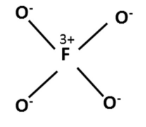
\includegraphics[width=0.2\linewidth]{Immagini/FO4.png}
        \caption{eventuale diagramma di $\textnormal{FO}_4^-$}
        \label{fig:FO4}
    \end{figure}
\end{ex}
Altri composti sono instabili a causa della riluttanza degli atomi del terzo (e successivo) periodo a formare legami multipli. I legami multipli sono limitati ad un numero ristretto di atomi di piccole dimensioni ed elevata elettronegatività, mentre difficilmente coinvolgono elementi di dimensioni maggiori e di minore elettronegatività. Questo può essere razionalizzato considerando che la diminuzione di elettronegatività (che diminuisce scendendo lungo un gruppo) comporta una diminuzione della capacità di confinare densità elettronica lungo
l'asse di legame.
\begin{ex}[\ce{CO2} e \ce{SiO2}]
    La preferenza di elementi del terzo gruppo (e successivi) a formare legami doppi ha conseguenze importanti. Ad esempio si può spiegare in questo modo il fatto che il diossido di carbonio $\text{CO}_2$ sia un gas, mentre il corrispondente composto $\text{SiO}_2$ sia un solido. La preferenza di Si a formare legami singoli rispetto a legami doppi, fa si che ciascun ossigeno sia in grado di legarsi ad altri atomi di Si dando origine al reticolo di un solido covalente polare. 
\end{ex}

\section{Legami intermolecolari}
Molecole discrete possono dare origine ad interazioni di legame, dette intermolecolari. Queste interazioni sono in genere più deboli delle interazioni di legame che uniscono atomi in molecole, ma sono di grande importanza in quanto determinano ad esempio lo stato di aggregazione di una sostanza e molte delle sue caratteristiche chimico-fisiche. Le forze di attrazione saranno relativamente forti tra molecole dotate di forti momenti di dipolo. Con buona approssimazione la forza di interazione può essere considerata come puramente elettrostatica. La presenza di forze intermolecolari rende conto dell'esistenza di liquidi e solidi.

Le uniche interazioni possibili tra molecole non polari sono interazioni di tipo Van der Waals, che possono essere attrattive o repulsive.
\begin{defn}[forze di van der Waals]
    Con il termine ``forza di van der Waals'' si includono tre tipo di interazioni intermolecolari:
    \begin{enumerate}
        \item forza dipolo permanente-dipolo permanente (o interazione di Keesom);
        \item forza dipolo permanente-dipolo indotto (o forza di Debye);
        \item forza dipolo istantaneo-dipolo indotto (o forza di dispersione di London).
    \end{enumerate}
    Queste includono anche il legame ione-dipolo, il legame ad alogeno e il legame ad idrogeno (la più forte delle interazioni di Keesom).
\end{defn}
nel caso di due atomi di elio l'approssimarsi dei due atomi genera una distorsione della distribuzione della densità elettronica, in altri termini una polarizzazione. Nel caso dei due atomi di gas inerte che si sta considerando, i momenti di dipolo elettrico mediati nel tempo sono nulli, ma è possibile pensare che a causa del moto delle cariche elettroniche in un istante qualunque sia presente un dipolo istantaneo $\bm{p_1}$. Questo momento di dipolo su un atomo in un certo istante $t$ produce un campo elettrico $E$ di ampiezza $2\bm{p_1}/R^3$ al centro del secondo atomo ad una distanza $R$ dal primo. Questo campo induce in quell'istante un momento di dipolo $\bm{p_2}=2\alpha\bm{p_1}/R^3$ sul secondo atomo in cui $\alpha$ è la polarizzabilità elettronica che dipende dal numero di elettroni e dalle dimensioni atomiche. L'energia potenziale dei due momenti di dipolo è data da
\begin{equation}
    V(r)\approx-\frac{2p_1p_2}{R^3}=-\frac{4\alpha p_1^2}{R^6}
\end{equation}
A causa del fattore $R^{-6}$ l'interazione aumenta rapidamente al diminuire della distanza, tuttavia, per distanze tali per cui si ha sovrapposizione delle densità elettroniche dei due atomi, entrambi con orbitali elettronici completi, il principio di esclusione di Pauli determina la repulsione dei due atomi e previene la formazione di un legame chimico. Le energie di legame associate alle forze di van der Waals sono circa due ordini di grandezza inferiori a quelle di un legame ionico o covalente. 

\section{Legame metallico}
In generale un metallo è caratterizzato da proprietà chimiche e fisiche particolari quali l'elevata conducibilità elettrica e termica, duttilità, malleabilità e caratteristico lustro e la tendenza a dare origine a specie cationiche in soluzione. Gli elementi metallici mostrano tuttavia una grande variabilità in altre proprietà, come ad esempio la densità. Lo stato metallico è caratterizzato dalla presenza di elettroni non legati, ovvero liberi di muoversi ad esempio in presenza di una differenza di potenziale. 

La natura del legame metallico può essere illustrata considerando ad esempio un insieme di atomi di cesio ad una distanza media sufficientemente grande da far si che l'elettrone di valenza $6s$ sia fermamente legato al suo nucleo atomico. Il sistema in queste condizioni non conduce elettricità, in quanto ciascun elettrone è legato. Secondo una visione classica l'atomo di cesio può essere visto come una molla che lega l'elettrone di valenza al suo ione parente $\text{Cs}^+$. La forza di legame dell'elettrone di valenza può essere paragonata alla rigidità della molla e quindi dalle oscillazioni caratteristiche che l'elettrone compie rispetto alla sua posizione di equilibrio. Nel regime di bassa densità (ovvero nel caso di atomi isolati) l'elettrone di valenza si muoverà poco dalla sua posizione di equilibrio. In altri termini la sua polarizzabilità sarà relativamente piccola. Aumentando la densità del sistema e muovendosi verso lo stato liquido o solido, si avrà una progressiva diminuzione della rigidità della molla a causa della mutua interazione tra i diversi atomi di cesio. Questo processo porta ad una riduzione della caratteristica frequenza di oscillazione dell'elettrone $6s$ e comporta spostamenti sempre più marcati dalla posizione di equilibrio dell'elettrone dal suo nucleo atomico. A densità sufficientemente elevate sufficientemente piccole si avrà una situazione detta di ``catastrofe di polarizzazione'', dove ciascun elettrone di valenza si stacca dal suo nucleo ed è può partecipare al processo di conduzione elettrica. Inoltre più l'elettronegatività è bassa maggiore sarà la distanza interatomica a cui la catastrofe di polarizzazione avrà luogo.
\begin{obs}
    L'elettronegatività di un elemento può essere usata come indicatore della natura metallica di un elemento: elementi con $\chi<1.9$ sono metallici, mentre con $\chi>1.9$ non lo sono.
\end{obs}
\begin{ex}[idrogeno metallico]
    L'idrogeno con configurazione $1s^1$ analoga a quella dei metalli alcalini, potrebbe essere atteso dare origine a un legame metallico, tuttavia l'elevato valore di elettronegatività $\chi=2.3$ comporta che l'elettrone di valenza sia fortemente legato al nucleo. La distanza tra un insieme di atomi di idrogeno che può dare luogo ad una catastrofe di polarizzazione è essere estremamente piccola. In effetti l'idrogeno dà origine ad uno stato metallico a pressioni estreme.
\end{ex}

\section{Teoria acido base}
Vi sono varie teorie che definiscono acidi e basi, le più significative sono: quella di Arrhenius, quella di Br\o nsted e Lowry e quella di Lewis.
\begin{defn}[acido e base di Arrhenius]\hfill
    \begin{itemize}
        \item Un acido è una sostanza che libera in soluzione acquosa ioni \textnormal{H}$_3$\textnormal{O}$^+$.
        \item Una base è una sostanza che libera in soluzione acquosa ioni \textnormal{OH}$^-$.
    \end{itemize}    
\end{defn}
\begin{ex}[Arrhenius] Un esempio di acido è $\ce{HCl}$ che soddisfa la reazione $\ce{HCl}+\ce{H2O}\to\ce{H+}+\ce{Cl-}$, mentre una base da $\ce{NaOH}$ che soddisfa la reazione $\ce{NaOH}+\ce{H2O}\to\ce{Na+}+\ce{OH-}$.
\end{ex}
\begin{defn}[acido e base di Br\o nsted e Lowry]\hfill
    \begin{itemize}
        \item Un acido è una sostanza che in una reazione dona uno ione \textnormal{H}$^+$.
        \item Una base è una sostanza che in una reazione accetta uno ione \textnormal{H}$^+$.
    \end{itemize}    
\end{defn}
\begin{ex}[Br\o nsted e Lowry] Un esempio di acido è $\ce{HCl}$ che soddisfa la reazione $\ce{HCl}+\ce{H2O}\to\ce{H3O}+\ce{Cl-}$, mentre una base da $\ce{O^2-}$ che soddisfa la reazione $\ce{O^2-}+\ce{H2O}\to\ce{OH-}+\ce{OH-}$.
\end{ex}
\begin{defn}[acido e base di Lewis]\hfill
    \begin{itemize}
        \item Un acido è una sostanza che in una reazione accetta una coppia di elettroni.
        \item Una base è una sostanza che in una reazione dona una coppia di elettroni.
    \end{itemize}
\end{defn}
\begin{ex}[Lewis] Un esempio di acido è $\ce{BF_3}$, mentre una base è $\ce{NH_3}$.
\end{ex}
\begin{obs}
    La definizione di Arrhenius ha il limite di riferirsi alle sole soluzioni acquose mentre numerose sostanze si comportano da acidi o da basi anche in situazioni diverse.
\end{obs}

\subsection{Reazioni di ossido-riduzione}
Il termine ``ossidazione'' originariamente veniva riferito alla combinazione di una sostanza con l'ossigeno, processo che comporta l'aumento del numero di ossidazione di un elemento della sostanza.
\begin{ex}
    La formazione della ruggine corrisponde alla seguente reazione $4\textnormal{Fe}_{\left(s\right)}+3{\textnormal{O}_2}_{\left(g\right)}\to2\textnormal{Fe}_2{\textnormal{O}_3}_{\left(s\right)}$, dove il numero di ossidazione di Fe passa da 0 a +3.
\end{ex}
Invece, originariamente la ``riduzione'' descriveva la rimozione di ossigeno da un composto. Ora i termini riduzione e ossidazione sono applicati in modo più generale.
\begin{defn}[riduzione e ossidazione]\hfill
    \begin{itemize}
        \item L'ossidazione consiste in un aumento del numero di ossidazione e corrisponde alla perdita, anche apparente, di elettroni.
        \item La riduzione consiste in una diminuzione del numero di ossidazione e corrisponde all'acquisto, anche apparente, di elettroni.
    \end{itemize}
\end{defn}
In una reazione gli elettroni non vengono né creati né distrutti, quindi riduzione e ossidazione avvengono simultaneamente e nella stessa misura.
\begin{axiom}[metodo del numero di ossidazione]
    Per bilanciare una reazione redox si segue il metodo del numero di ossidazione che consiste in:
    \begin{enumerate}
        \item assegnare il numero di ossidazione agli elementi che partecipano alla redox;
        \item bilanciare (se necessario) gli elementi che partecipano alla redox;
        \item calcolare il numero di elettroni trasferiti per ogni unità formula;
        \item assegnare i coefficienti stechiometrici all'agente ossidante e all'agente riducente in modo da uguagliare il numero di elettroni ceduti ed acquistati;
        \item bilanciare gli elementi rimanenti secondo la legge di Lavoisier.
    \end{enumerate}
\end{axiom}
\begin{ex}
    Un esempio di reazione di redox è la seguente
    \begin{equation}
        \textnormal{K}_2\textnormal{Cr}_2\textnormal{O}_7+\textnormal{H}_2\textnormal{O}+\textnormal{S}\to\textnormal{SO}_2+\textnormal{KOH}+\textnormal{Cr}_2\textnormal{O}_3.
    \end{equation}
    Si procede secondo le regole elencate prima:
    \begin{enumerate}
        \item Il numero di ossidazione di \textnormal{S} passa da 0 a +4, mentre quello del \textnormal{Cr} da +6 a +3.
        \item In questo caso non è necessario bilanciare \textnormal{S} e \textnormal{Cr}.
        \item Ogni unità di formula \textnormal{K}$_2$\textnormal{Cr}$_2$\textnormal{O}$_7$ contiene due atomi di \textnormal{Cr}, ognuno dei quali acquista 3 elettroni, in totale 6. Ogni atomo di \textnormal{S} perde 4 elettroni.
        \item Affinché gli elettroni ceduti ed acquistati siano in egual numero, è necessario far reagire 2 unità formula di \textnormal{K}$_2$\textnormal{Cr}$_2$\textnormal{O}$_7$ con 3 atomi di \textnormal{S}. Questo si indica ponendo come coefficiente di \textnormal{K}$_2$\textnormal{Cr}$_2$\textnormal{O}$_7$ e \textnormal{Cr}$_2$\textnormal{O}$_3$ un fattore 2, e un fattore 3 davanti a \textnormal{S} e \textnormal{SO}$_2$.
        \item Per la legge di Lavoisier si completa il bilanciamento in modo usuale.
    \end{enumerate}
    Dunque, si ottiene
    \begin{equation}
        2\textnormal{K}_2\textnormal{Cr}_2\textnormal{O}_7+2\textnormal{H}_2\textnormal{O}+3\textnormal{S}\to3\textnormal{SO}_2+4\textnormal{KOH}+2\textnormal{Cr}_2\textnormal{O}_3.
    \end{equation}
\end{ex}

\section{Cenni di nomenclatura}
Si elencano delle regole di nomenclatura di alcuni composti binari e ternari.
\subsubsection{Composti ionici}
\begin{enumerate}
    \item Cationi: mantengono il nome dell'elemento e si riporta il numero di ossidazione usando i numeri romani. 
    \begin{ex} $\ce{Fe}^{2+}$ è Ferro II e $\ce{Fe}^{3+}$ è Ferro III.
    \end{ex}
    \item Ioni positivi: prendono il suffisso -onio.
    \begin{ex}
        $\ce{NH}_4^+$ è lo ione ammonio e $\ce{N3O+}$ è lo ione idronio.
    \end{ex}
    \item Anioni: prendono il suffisso -uro, ad eccezione dell'anione O$^{2-}$ che è ossido.
    \begin{ex}
         $\ce{H-}$ è lo ione idruro e $\ce{Cl-}$ è lo ione cloruro.
    \end{ex}
    \item Ioni negativi: prendono il suffisso -uro dopo il nome dell'elemento, ad eccezione di OH$^-$ che idrossido.
    \begin{ex}
        $\ce{CN-}$ è lo ione cianuro.
    \end{ex}
\end{enumerate}
\subsubsection{Composti binari}
\begin{enumerate}
    \item Sali binari: prendono il nome dal non-metallo con suffisso in -uro seguito dal nome del metallo.
    \begin{ex}
        $\ce{FeCl2}$ è dicloruro di ferro (II).
    \end{ex}
    \item Ossidi (basici e acidi): prendono il nome di ossido, con eventuale prefisso, seguito dal nome del metallo (non-metallo).
    \begin{ex}
        $\ce{Na2O}$ è ossido di sodio e  $\ce{Fe2O3}$ è triossido di diferro.
    \end{ex}
    \item Perossidi: il gruppo perossido è O$_2^{2-}$.
    \begin{ex} 
        $\ce{H2O2}$ è perossido di idrogeno.
    \end{ex}
    \item idruri (idracidi): prendono il nome di idruro, con eventuale prefisso, seguito dal nome del particolare elemento (solo VI e VII gruppo).
    \begin{ex}
        $\ce{LiH}$ è idruro di litio.
    \end{ex}
\end{enumerate}
\subsubsection{Composti ternari}
\begin{enumerate}
    \item Idrossidi (ossido basico + H$_2$O): prendono il nome di idrossido, con eventuale prefisso, seguito dal nome del metallo.
    \begin{ex}
        $\ce{Mg(OH)2}$ è idrossido di magnesio.
    \end{ex}
    \item Ossiacido (ossido acido + H$_2$O): prendono il nome di acido seguito da \textnormal{n° atomi di ossigeno + osso + n° atomi non-metallo + radice + -ico + (n° ox. non-metallo)}.
    \begin{ex}
        $\ce{HClO}$ è acido monoossoclorico (I).
    \end{ex}
\end{enumerate}
La forza di un ossiacido è determinata dal numeri di ossigeni: maggiore è il numero di ossigeni tanto più sarà delocalizzata la carica e stabile (debole) la base coniugata. Di conseguenza tanto più forte sarà l'acido
\begin{ex}
    I seguenti acidi soddisfano questa relazione relativa alla forza di ciascuno: $\textnormal{HClO}_4>\textnormal{HClO}_3>\textnormal{HClO}_2>\textnormal{HOCl}$.
\end{ex}